\documentclass[12pt,fleqn]{article}
\setlength{\parindent}{0pt}
\usepackage{graphicx}
\usepackage{cancel}
\usepackage{listings}
\usepackage[latin5]{inputenc}
\usepackage{color}
\setlength{\parskip}{8pt}
\setlength{\parsep}{0pt}
\setlength{\headsep}{0pt}
\setlength{\topskip}{0pt}
\setlength{\topmargin}{0pt}
\setlength{\topsep}{0pt}
\setlength{\partopsep}{0pt}
\setlength{\mathindent}{0cm}

\begin{document}
Cok Degiskenli Calculus - Ders 21

Bir onceki ders yol bagimsizligi ozelligi ve muhafazakarligin birebir
iliskide oldugunu gorduk. Bu derste bir alana bakarak o alanin gradyan
alani olup olmadigini anlamamizi saglayacak bir matematiksel kriter
gorecegiz, ve eger alan bir gradyan alani ise, onun bagli oldugu potansiyel
alani hesaplamanin yolunu isleyecegiz. 

Bir vektor alani $\vec{F} = <M,N>$ eger gradyan alani ise 

\[ M = f_x \]

\[ N = f_y \]

Bunu biliyoruz. Kismi turevlerin daha once ogrendigimiz ozelligine
gore, sunu da biliyoruz. $f_{xy} = f_{yx}$ mesela. O zaman elimizde bir
gradyan alani var ise

\[ M_y = N_x \]

dogru olmali. 

Tek kontrol etmemiz gereken bu. Tabii vektor alani $\vec{F} = <M,N>$ her
yerde tanimli ve turevi alinabilir bir formda olmali. Tanimlilik hakkinda -
odevlerimizden birisi bu konuyu isliyor mesela, size tek bir nokta
haricinde her yerde tanimli bir vektor alani veriyoruz, ve tum bu
anlattiklarimiz o noktada ise yaramaz hale geliyor. Bu konuyu daha derin
sekilde inceleyecegiz, mesela ``basit sekilde bagli bolgeler (simply
connected regions)'' konusuna bakacagiz. 

Simdilik su yeterli, eger alan her yerde tanimli ise ve $M_y = N_x$ ise,
alan bir gradyan alanidir. 

Ornek 

\[ \vec{F} = -y\hat{i} + x\hat{j} \]

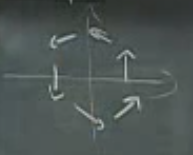
\includegraphics[height=3cm]{21_1.png}

















\end{document}
